
\pagebreak	
\section{Scheduling}
\label{bkm:Ref445400921}
In the current CUBE PA version you can upload schedules (as PDF files) and make them accessible to project staff who use CUBE PA. Two schedules were imported and made available in the present documentation: complete scheduling program and and study contract procedure of the WB train station. \\
As a second function of scheduling, you can import complex schedules created with Microsoft Project as .xml files and then filter them in CUBE PA and generate user-specific views.

%Die Terminplanung beschränkt sich in dern aktuellen CUBE PA Version auf das Herunterladen des Gesamtterminprogramms und das Studienauftragsverfahren Bhf WB, sowie die Filterung und entsprechenden Anzeige des Detailterminprogramms.

\subsection{The scheduling view}

\begin{wrapfigure}[8]{l}{6.5cm}   % [x] Wie manche Zeile soll sich um die Grafik "brechen"
  \vspace{-35pt}      % Grundwert war 20; mit 30 schön oben beim Text ausgerichtet
  \begin{center}
    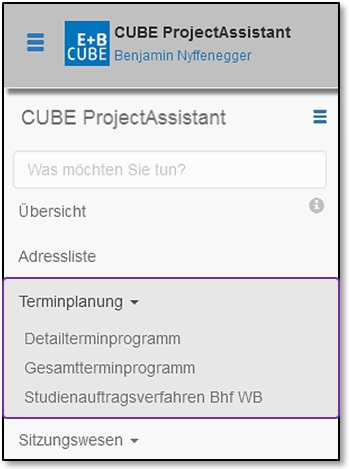
\includegraphics[width=1\linewidth]{../chapters/04_Terminplanung/pictures/4-1_Menu_Terminplanung.jpg}
  \end{center}
  \vspace{-20pt}
  \caption{Using the scheduling function}
  \vspace{-10pt}
\end{wrapfigure}

In the left-hand menu, select the menu item 'Scheduling' and then the desired subcategory. (By clicking on 'Scheduling', the sub-items are shown and hidden). In the scheduling function you can add customer-specific schedules. This means that the menu may look different to you than how it does in the documentation.

\vspace{5cm} 

\subsection{The complete scheduling program and the study contract procedure of the WB train station}

Both these functions are about downloading the corresponding scheduling program.\newline
When you select the subcategory 'Complete scheduling program' under 'Scheduling' in the menu, the following view appears (this view depends on the CUBE PA configuration):
% kundenspezifisch
\begin{figure}[H]
\center{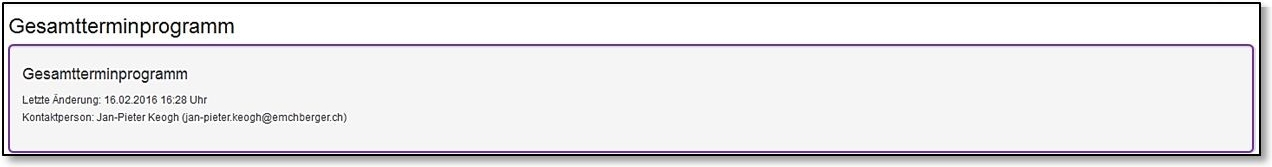
\includegraphics[width=1\linewidth]{../chapters/04_Terminplanung/pictures/4-2_Gesamtterminprogramm.jpg}}
\caption{Complete scheduling program}
% \label{fig:speciation}
\end{figure}

Click in the violet-framed area to download the complete scheduling program. In the next window, you can select whether the document is to be opened or saved at a certain location.

\vspace{\baselineskip}

When you select the subcategory 'Study contract procedure WB train station' under 'Scheduling' in the menu, the following view appears:

% kundenspezifisch
\begin{figure}[H]
\center{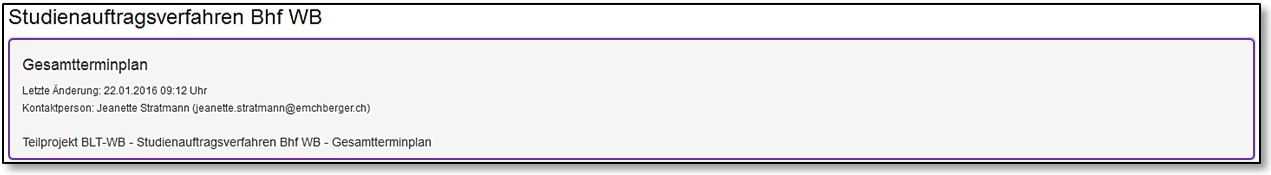
\includegraphics[width=1\linewidth]{42_Studienauftragsv.jpg}}
\caption{Study contract procedure WB train station}
% \label{fig:speciation}
\end{figure}

Click in the violet-framed area to download the study contract procedure of the WB train station. In the next window, you can select whether the document is to be opened or saved at a certain location.

\subsection{The detailed scheduling program}

Select the the subcategory 'Detailed scheduling program' under 'Scheduling' in the menu. The following window appears, in which you can select the desired filter settings:

\begin{figure}[H]
\center{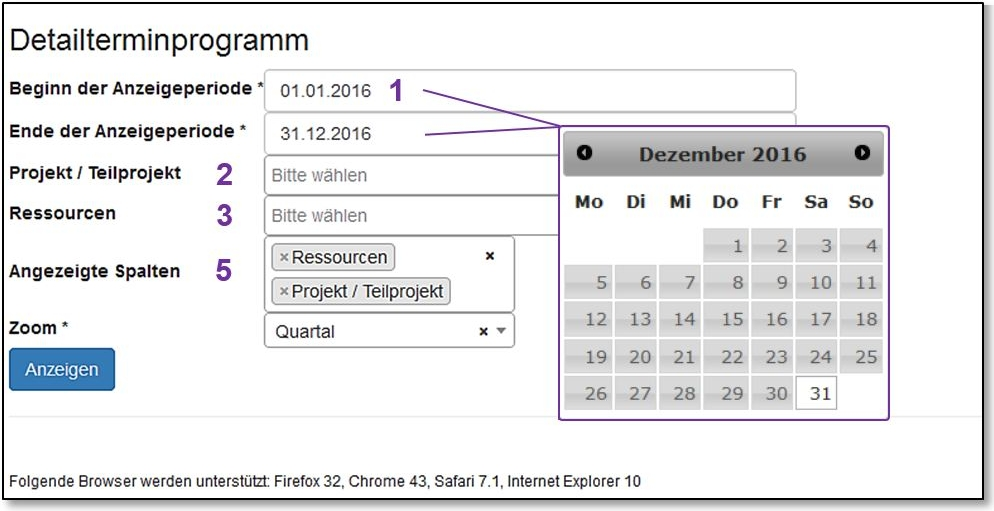
\includegraphics[width=.75\linewidth]{../chapters/04_Terminplanung/pictures/4-3_Detailterminprogramm.jpg}}
\caption{Detailed scheduling program}
% \label{fig:speciation}
\end{figure}

The fields marked with a * are mandatory fields where data must be selected. Choose the start and end of the period for which you want to view the schedule \col{(1)}. A calender view appear, in which you can select the desired date. You can optionally select a project / subproject \col{(2)} and also resources \col{(3)}.

\begin{figure}[H]
\center{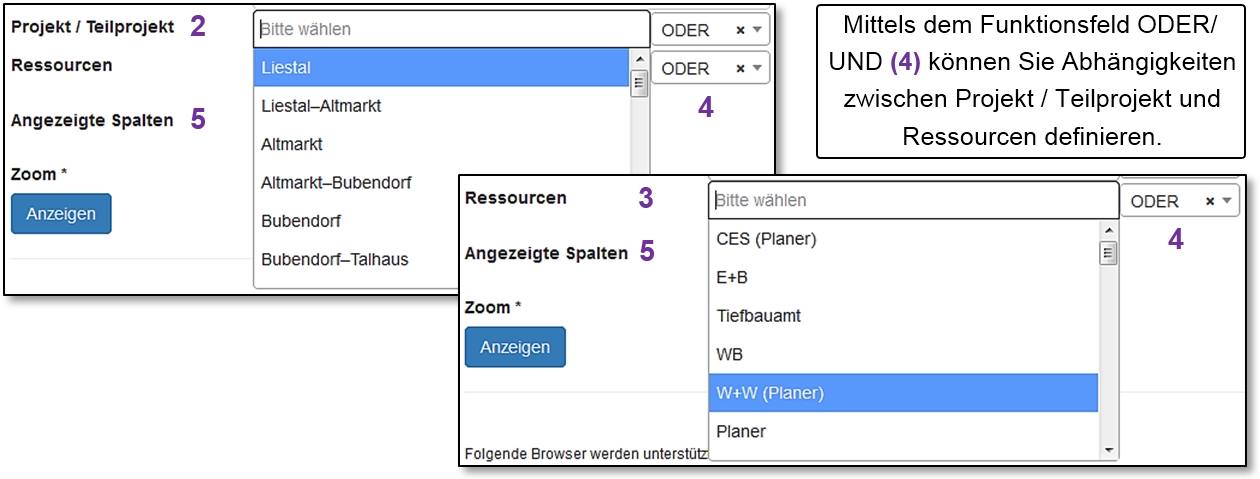
\includegraphics[width=1\linewidth]{../chapters/04_Terminplanung/pictures/4-3_Termine_Abhaengigkeiten.jpg}}
\caption{Defining dependencies}
% \label{fig:speciation}
\end{figure}

% Text als Grafik implementiert
% Mittels dem Funktionsfeld ODER/UND \textbf{\textcolor[rgb]{0.4392157,0.1882353,0.627451}{(4)}} können Sie Abhängigkeiten zwischen Projekt / Teilprojekt und Ressourcen definieren.

Select the columns (project / subproject, resources) to be displayed in the filter result \col{(5)}. You can also select a second column by clicking again in the 'Visible Columns' field. In order to filter by project / subproject or resources and to display the columns in the schedule, the corresponding information must be available in the MS Project file (see chapter \ref{bkm:Ref445411998}).

% Ref einfügen nach 12.1

\vspace{\baselineskip}

\begin{wrapfigure}[4]{r}{6cm}
  \vspace{-30pt}
  \begin{center}
    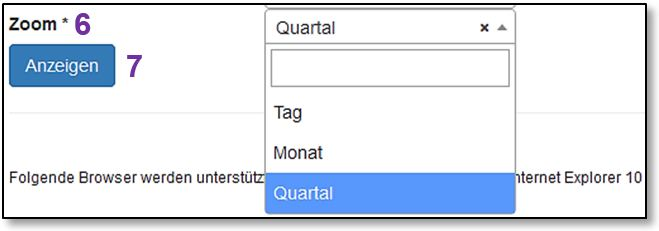
\includegraphics[height=25mm]{43_Zoom-Ansicht.jpg}
  \end{center}
  \vspace{-20pt}
  \caption{Zoom view}
  \vspace{-10pt}
\end{wrapfigure}
Under \col{(6)} you can select if you want a view of the day, month, or trimester. Once the desired filter settings are selected, click on 'Display' \col{(7)}.

\vspace{\baselineskip}
\vspace{\baselineskip}

After clicking on 'Display', the filtered result of the scheduling calendar is shown:

\begin{figure}[H]
\center{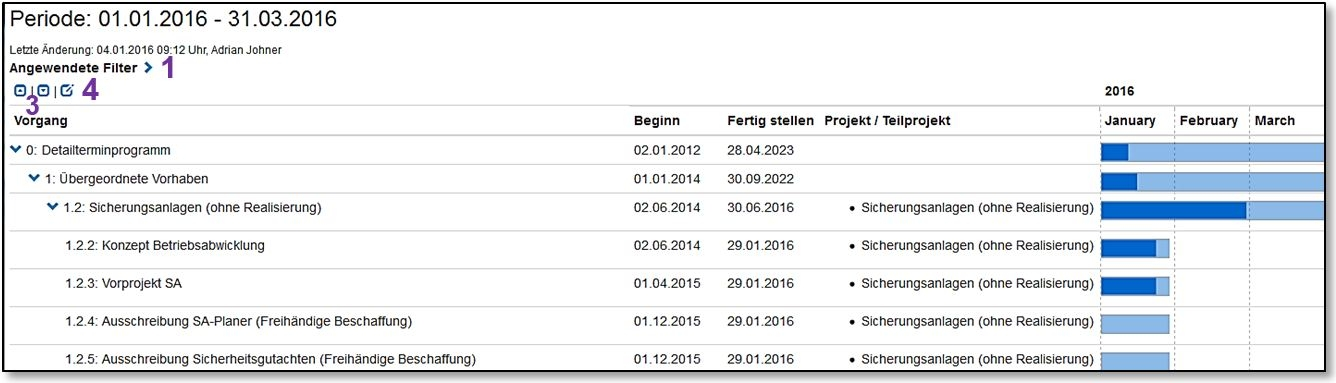
\includegraphics[width=1\linewidth]{43_Termin_Ergebnis.jpg}}
\caption{Result of the scheduling calendar}
% \label{fig:speciation}
\end{figure}

Clicking on the arrow 
\includegraphics[height=12pt]{/Icons/Pfeil_rechts.jpg} \col{(1)} shows the applied filter. Clicking on it again 
\includegraphics[height=12pt]{/Icons/Pfeil_unten.jpg} \col{(2)} hides the filter.

\begin{figure}[H]
\center{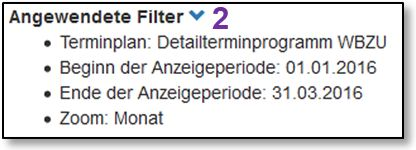
\includegraphics[width=.4\linewidth]{43_Termin_Filter.jpg}}
\caption{Applied filter}
% \label{fig:speciation}
\end{figure}

Using both arrows 
\includegraphics[height=12pt]{/Icons/Pfeil_auf-ab.jpg} \col{(3)} you can show and hide all the details. To adjust the filter settings, click on the editing symbol 
\includegraphics[height=12pt]{/Icons/Bearbeiten.jpg} \col{(4)}.
